\documentclass{standalone}

\begin{document}


\documentclass{standalone}

\begin{document}

\chapter[Deep Learning]{Deep Learning - Neural Network algorithms}\label{chapter2:neural}

In the first chapter we have discussed about the difficulties on extracting information from a huge amount of data, and we have proposed a novel feature selection algorithm to face these problems.
Those kind of applications go under the wide research field of Machine Learning.
Machine learning algorithms are closely related to a statistical interpretation of the available data.
With the increasing availability of computational power and data it is not always possible to tune and build an accurate model able to describe the heterogeneity of our samples.
Many everyday problems involve very complex tasks, and we are interested on models able to solve many tasks at the same time.
From a machine learning point-of-view this can be achieved building pipelines, i.e work-flows made by multiple steps of processing, which aim to simulate as much close as possible the human intelligence.
This leads us into the Deep Learning research field, in which very computational expensive models have been built to face general purpose problems, often related to real time applications.

The description of a deep learning model is quite often given by a Neural Network architecture, i.e a more or less complex pipeline of functions which takes in input a sample and it applies a series of transformations and filters to obtain the required result.
All these pipelines are very computational expensive and they require appropriate optimization strategies.

In this chapter we introduce some of the most common functions related to deep learning applications, giving a very fast mathematical explanation of them and carefully focusing on their numerical issues and solutions.
We start from an introduction about general Neural Network models up to some of modern deep learning models, involving object detection, image segmentation and image super resolution.
In particular, we describe two custom libraries (\textsf{NumPyNet} and \textsf{Byron}) developed by the author of this thesis, for educational and analytical purposes, respectively.
Both libraries are released with MIT license and the codes are publicly available on my Github page (\href{https://github.com/Nico-Curti/Byron}{Byron} and \href{https://github.com/Nico-Curti/NumPyNet}{NumPyNet}).
These libraries have already used in several applications and in the last sections we show some of the obtained results\footnote{
  Both \textsf{NumPyNet} and \textsf{Byron} libraries have been developed with the collaboration of master degree students and several thesis have their applications as core arguments.
}.

In the last section of this chapter we introduce a different kind of Neural Network model, the \textsf{Replicated Focusing Belief Propagation} (rFBP) model.
This model has solid physical and statistical bases and we discuss about its novel optimized implementation, available on my Github (\href{https://github.com/Nico-Curti/rFBP}{Replicated Focusing Belief Propagation}) and released under MIT license.
This model differs from standard deep learning neural networks changing the updating rule and we show its first application on real data.

\end{document}
 % Neural Network introduction

\documentclass{standalone}

\begin{document}

\section[Fully Connected]{Fully Connected Neural Network}\label{connected}

The fundamental unit of each Neural Network model is the \emph{simple Perceptron} (or single neuron).
The \emph{Perceptron} it the simpler mathematical model of biological neuron and it is based on the Rosenblatt~\cite{Rosenblat} model which identifies a neuron as a computational unit with input, synaptic weights and an activation threshold (or function).
Following the biological model of Hodgkin and Huxley~\cite{HHmodel} (H-H model), we have an action potential, i.e the output of the neuron, given by

$$
y = \sigma\left(\sum_{i=1}^{N}w_i x_i + w_0 \right)
$$
\\
where $\sigma$ is the activation function, $w_i$ are the synaptic weights and $x_i$ the inputs.
The $w_0$ coefficient identifies the bias of the linear combination and it is left as parameter to be tune by the optimization algorithm.

The connection weights $w_i$ are tuned during the training section by the chosen updating rule.
The standard updating rule is simply given

$$
w_i(\tau + 1) = w_i(\tau) + \gamma(t - y)x
$$
\\
where $\gamma$ is the gain or step size ($\gamma \in [0, 1]$) and $t$ is the desired output.
In other words we have to firstly compute the difference between the current output and the desired one, i.e the error, and weight this error by the gain factor and the corresponding input.
Repeating the error computation and the updating rule we can bring the weights to convergence.
From a geometrical point-of-view this process is equivalent to an hyper-plane placement defined by $w_0 + < w, x >$ which splits an $n-$dimensional space into two half-spaces, i.e two desired classes.

The mathematical formulation already highlights the numerous limits of this model.
The output function is a simple linear combination of the input with a vector of weights and so only linearly separable problems can be learned by the \emph{Perceptron}\footnote{
  A classical example of learning problems is given by the XOR logic function.
  Since the XOR output is not linearly separable the Perceptron could not converge.
}.
Moreover we can manage only two classes since an hyper-plane divide the space in only two half-spaces.

To overcome these problems we can join together multiple Perceptron units into a more complex network of interaction in which the output of a neuron feed-forward the input of an other.
This is the Multi-layers Perceptron (MLP) configuration and if the graph is fully connected, i.e each neuron is connected to all the others, we talk about \emph{fully connected neural networks} (or \emph{dense} neural network, DNN).

Given the Perceptron formulas, the extrapolation to the MLP architecture is straight-forward and given by

$$
y = \sigma\left(X \cdot W + W_0 \right)
$$
\\
where we simply pass from the vector formulation to the matrix one.
The updating rule consequentially becomes

$$
W(\tau + 1) = W(\tau) + \gamma X^T (T - Y)
$$
\\
where also in this case we simply pass to the matrix formalism.
From the re-iteration of such structures we can join together multiple fully connected layers and so obtain multiple neuron layers jointly together with different levels of complexity and units (an input layer followed by multiple \emph{hidden} layers).

The fully connected Neural Networks overcome the told above \emph{Perceptron} problems using a combination of linear functions (single \emph{Perceptron} units) and they gain more useful properties:

\begin{itemize}

\item If the activation functions of \emph{all} the hidden units in the Neural Network are linear, then the network architecture is equivalent to a network without hidden units.

\item If the number of hidden units is smaller than either the number of input units either the number of output ones, then the network can generate transformations from inputs to outputs as much general as possible since the information is lost in the dimensionality reduction performed by the hidden units.

\item We can find multiple weight configurations, i.e $W$ matrices, which give us the same mapping function from inputs to outputs.

\end{itemize}

%% Aggiungere parte sulla back-propagation

\end{document}

\documentclass{standalone}

\begin{document}


\subsubsection[Matrix Product]{Matrix Product}\label{NN:gemm}

Despite the mathematical formulation of the model we have to take in count also an efficient implementation.
From a numerical point-of-view we can notice that all the computation required by this kind of Networks (or layer if we consider it into an hybrid Neural Network architecture as we will see in the next sections) can be summarized into the matrix product evaluation.
The matrix product is a well-known numerical problems and the complexity of the algorithm can be hardly reduced under $O(N^3)$\footnote{
  The complexity is often given in the assumption of only square matrices $(N\times N)$ involved in the computation.
  For no-square matrix the algorithm complexity is given by the product of the three possible different matrix dimensions involved ($(N\times K) = (N\times M)(M\times K)$ brings to $O(NMK)$ complexity).
  More sophisticated implementation of the algorithm are able to reduce the algorithm complexity (e.g Strassen algorithm) but neither implementation is able to overcome the $O(N^{2.7})$ complexity up-to-now.
}.
A crucial role on this kind of algorithms is played by the cache accesses.
The CPU cache is the hardware cache used by the CPU to store small portion of data in order to reduce the average cost (in time or energy consumption) to data access from the main memory.
Cache optimization is one of the most difficult parts to perform writing an algorithm, but can lead to highest performance gains.

In the matrix product we have to multiply each row of a matrix $A$ by each column of a second matrix $B$.
We work in the assumption that each matrix is stored into an array of 1D or 2D without nested structures.
In this case we can access to a contiguous memory portion of the first matrix since each row will be given by a series of sequential index locations (the row elements will be given by $x[0], x[1], \dots, x[N]$).
This configuration allows the cache optimization in the access to the first matrix since we can store in the small portion of cache memory a series of row elements and use them in a vectorization environment.

From the second matrix we have to extract the elements from each column.
This means that the elements will be given by a discontinuous portion of memories (the column elements will be given by $x[0], x[M], x[2M], \dots, x[N(M-1)]$).
In this case we can not insert a full column into the cache memory and in consequence we will have a \emph{cache-miss} at each iteration\footnote{
  The \emph{cache-miss} happens when a required data can not be found into the cache and so its search has to be done in the main memory (RAM).
}.

The simple matrix product as given by row-column multiplication is already affected by an intrinsic numerical problem which can drastically affect its performances.
The simplest workaround of this problem is to perform a transposition of the second matrix to obtain a row-row matrix product\footnote{
  In the discussion we have silently ignored the problems of matrix storage and the cache optimization for the resulting matrix accesses but in the above discussion we want to focus only on the main problems raising from the matrix product.
}.
In this way both matrices can be accessed in a sequential order.
The total complexity of the computation increase to $O(N^2)$ (for the matrix transposition, in the better case) $+ O(N^3)$ (for matrix product) but the numerical performances increase due to the cache-miss minimization\footnote{
  The cache memory is a very tight portion of memory and it is impossible to completely remove cache-misses.
}.

Following back to our Neural Network implementation we can obtain the output values using the above technique.
Moreover we can assumes from the beginning that the weight matrix is transposed and so remove the transposition step from the matrix product.
This simple (but carefully studied) optimization allows us to obtain better results in the feed-forward evaluation but it paybacks a revision of the standard mathematical formulation and a carefully implementation of the code.

\begin{figure}[htbp]
\includegraphics[width=0.45\textwidth]{gemm_schema.png}
\quad
\centering
\def\svgwidth{0.45\textwidth}
\documentclass{standalone}

\begin{document}


\subsubsection[Matrix Product]{Matrix Product}\label{NN:gemm}

Despite the mathematical formulation of the model we have to take in count also an efficient implementation.
From a numerical point-of-view we can notice that all the computation required by this kind of Networks (or layer if we consider it into an hybrid Neural Network architecture as we will see in the next sections) can be summarized into the matrix product evaluation.
The matrix product is a well-known numerical problems and the complexity of the algorithm can be hardly reduced under $O(N^3)$\footnote{
  The complexity is often given in the assumption of only square matrices $(N\times N)$ involved in the computation.
  For no-square matrix the algorithm complexity is given by the product of the three possible different matrix dimensions involved ($(N\times K) = (N\times M)(M\times K)$ brings to $O(NMK)$ complexity).
  More sophisticated implementation of the algorithm are able to reduce the algorithm complexity (e.g Strassen algorithm) but neither implementation is able to overcome the $O(N^{2.7})$ complexity up-to-now.
}.
A crucial role on this kind of algorithms is played by the cache accesses.
The CPU cache is the hardware cache used by the CPU to store small portion of data in order to reduce the average cost (in time or energy consumption) to data access from the main memory.
Cache optimization is one of the most difficult parts to perform writing an algorithm, but can lead to highest performance gains.

In the matrix product we have to multiply each row of a matrix $A$ by each column of a second matrix $B$.
We work in the assumption that each matrix is stored into an array of 1D or 2D without nested structures.
In this case we can access to a contiguous memory portion of the first matrix since each row will be given by a series of sequential index locations (the row elements will be given by $x[0], x[1], \dots, x[N]$).
This configuration allows the cache optimization in the access to the first matrix since we can store in the small portion of cache memory a series of row elements and use them in a vectorization environment.

From the second matrix we have to extract the elements from each column.
This means that the elements will be given by a discontinuous portion of memories (the column elements will be given by $x[0], x[M], x[2M], \dots, x[N(M-1)]$).
In this case we can not insert a full column into the cache memory and in consequence we will have a \emph{cache-miss} at each iteration\footnote{
  The \emph{cache-miss} happens when a required data can not be found into the cache and so its search has to be done in the main memory (RAM).
}.

The simple matrix product as given by row-column multiplication is already affected by an intrinsic numerical problem which can drastically affect its performances.
The simplest workaround of this problem is to perform a transposition of the second matrix to obtain a row-row matrix product\footnote{
  In the discussion we have silently ignored the problems of matrix storage and the cache optimization for the resulting matrix accesses but in the above discussion we want to focus only on the main problems raising from the matrix product.
}.
In this way both matrices can be accessed in a sequential order.
The total complexity of the computation increase to $O(N^2)$ (for the matrix transposition, in the better case) $+ O(N^3)$ (for matrix product) but the numerical performances increase due to the cache-miss minimization\footnote{
  The cache memory is a very tight portion of memory and it is impossible to completely remove cache-misses.
}.

Following back to our Neural Network implementation we can obtain the output values using the above technique.
Moreover we can assumes from the beginning that the weight matrix is transposed and so remove the transposition step from the matrix product.
This simple (but carefully studied) optimization allows us to obtain better results in the feed-forward evaluation but it paybacks a revision of the standard mathematical formulation and a carefully implementation of the code.

\begin{figure}[htbp]
\includegraphics[width=0.45\textwidth]{gemm_schema.png}
\quad
\centering
\def\svgwidth{0.45\textwidth}
\documentclass{standalone}

\begin{document}


\subsubsection[Matrix Product]{Matrix Product}\label{NN:gemm}

Despite the mathematical formulation of the model we have to take in count also an efficient implementation.
From a numerical point-of-view we can notice that all the computation required by this kind of Networks (or layer if we consider it into an hybrid Neural Network architecture as we will see in the next sections) can be summarized into the matrix product evaluation.
The matrix product is a well-known numerical problems and the complexity of the algorithm can be hardly reduced under $O(N^3)$\footnote{
  The complexity is often given in the assumption of only square matrices $(N\times N)$ involved in the computation.
  For no-square matrix the algorithm complexity is given by the product of the three possible different matrix dimensions involved ($(N\times K) = (N\times M)(M\times K)$ brings to $O(NMK)$ complexity).
  More sophisticated implementation of the algorithm are able to reduce the algorithm complexity (e.g Strassen algorithm) but neither implementation is able to overcome the $O(N^{2.7})$ complexity up-to-now.
}.
A crucial role on this kind of algorithms is played by the cache accesses.
The CPU cache is the hardware cache used by the CPU to store small portion of data in order to reduce the average cost (in time or energy consumption) to data access from the main memory.
Cache optimization is one of the most difficult parts to perform writing an algorithm, but can lead to highest performance gains.

In the matrix product we have to multiply each row of a matrix $A$ by each column of a second matrix $B$.
We work in the assumption that each matrix is stored into an array of 1D or 2D without nested structures.
In this case we can access to a contiguous memory portion of the first matrix since each row will be given by a series of sequential index locations (the row elements will be given by $x[0], x[1], \dots, x[N]$).
This configuration allows the cache optimization in the access to the first matrix since we can store in the small portion of cache memory a series of row elements and use them in a vectorization environment.

From the second matrix we have to extract the elements from each column.
This means that the elements will be given by a discontinuous portion of memories (the column elements will be given by $x[0], x[M], x[2M], \dots, x[N(M-1)]$).
In this case we can not insert a full column into the cache memory and in consequence we will have a \emph{cache-miss} at each iteration\footnote{
  The \emph{cache-miss} happens when a required data can not be found into the cache and so its search has to be done in the main memory (RAM).
}.

The simple matrix product as given by row-column multiplication is already affected by an intrinsic numerical problem which can drastically affect its performances.
The simplest workaround of this problem is to perform a transposition of the second matrix to obtain a row-row matrix product\footnote{
  In the discussion we have silently ignored the problems of matrix storage and the cache optimization for the resulting matrix accesses but in the above discussion we want to focus only on the main problems raising from the matrix product.
}.
In this way both matrices can be accessed in a sequential order.
The total complexity of the computation increase to $O(N^2)$ (for the matrix transposition, in the better case) $+ O(N^3)$ (for matrix product) but the numerical performances increase due to the cache-miss minimization\footnote{
  The cache memory is a very tight portion of memory and it is impossible to completely remove cache-misses.
}.

Following back to our Neural Network implementation we can obtain the output values using the above technique.
Moreover we can assumes from the beginning that the weight matrix is transposed and so remove the transposition step from the matrix product.
This simple (but carefully studied) optimization allows us to obtain better results in the feed-forward evaluation but it paybacks a revision of the standard mathematical formulation and a carefully implementation of the code.

\begin{figure}[htbp]
\includegraphics[width=0.45\textwidth]{gemm_schema.png}
\quad
\centering
\def\svgwidth{0.45\textwidth}
\input{./img/gemm.pdf_tex}
\caption{GEMM algorithms time performances.
GEMM NN: matrix multiplication considering both the matrices in \quotes{normal} format, i.e $A\cdot B$.
GEMM NT: matrix multiplication considering the first matrix in \quotes{normal} format and the second one transposed, i.e $A\cdot B^T$.
We perform 100 tests of 1K runs each of both the gemm algorithms using the \textsf{einsum} function of Numpy library.
The values are rescaled according to the mean time of the GEMM NN algorithm.
}
\label{fig:gemm}
\end{figure}

In the proposed numerical implementations of this model we implement both the matrix product cases to compare the performance results.
We tested the two implementation inside Python using the \textsf{einsum} function provided by the Numpy package.
In particular we evaluate the timing performances over 1000 applications of two the gemm functions (GEMM NN, i.e considering both matrices in \quotes{normal} shapes; GEMM NT, i.e considering the first matrix as \quotes{normal} and the second transpose) considering matrices of shapes ($100\times100$).
We performed 500 run and we save the minimum time obtained over the 10 realizations.
In Fig.~\ref{fig:gemm} we show the results rescaled by the mean time of the GEMM NN algorithm (reference).
As can be seen in Fig.~\ref{fig:gemm} the speedup of the GEMM NT matrix is evident and it is always faster than GEMM NN algorithm with a maximum of 3.2x in the speedup.

In the Byron library implementation we provide a parallelized version of this algorithm with also an \textsf{avx} support.
In this way we could manually manage the register memory of the two matrices and obtain faster version of the GEMM algorithm (especially for dimensions proportional to powers of 2 which are very common in neural network models).

\end{document}

\caption{GEMM algorithms time performances.
GEMM NN: matrix multiplication considering both the matrices in \quotes{normal} format, i.e $A\cdot B$.
GEMM NT: matrix multiplication considering the first matrix in \quotes{normal} format and the second one transposed, i.e $A\cdot B^T$.
We perform 100 tests of 1K runs each of both the gemm algorithms using the \textsf{einsum} function of Numpy library.
The values are rescaled according to the mean time of the GEMM NN algorithm.
}
\label{fig:gemm}
\end{figure}

In the proposed numerical implementations of this model we implement both the matrix product cases to compare the performance results.
We tested the two implementation inside Python using the \textsf{einsum} function provided by the Numpy package.
In particular we evaluate the timing performances over 1000 applications of two the gemm functions (GEMM NN, i.e considering both matrices in \quotes{normal} shapes; GEMM NT, i.e considering the first matrix as \quotes{normal} and the second transpose) considering matrices of shapes ($100\times100$).
We performed 500 run and we save the minimum time obtained over the 10 realizations.
In Fig.~\ref{fig:gemm} we show the results rescaled by the mean time of the GEMM NN algorithm (reference).
As can be seen in Fig.~\ref{fig:gemm} the speedup of the GEMM NT matrix is evident and it is always faster than GEMM NN algorithm with a maximum of 3.2x in the speedup.

In the Byron library implementation we provide a parallelized version of this algorithm with also an \textsf{avx} support.
In this way we could manually manage the register memory of the two matrices and obtain faster version of the GEMM algorithm (especially for dimensions proportional to powers of 2 which are very common in neural network models).

\end{document}

\caption{GEMM algorithms time performances.
GEMM NN: matrix multiplication considering both the matrices in \quotes{normal} format, i.e $A\cdot B$.
GEMM NT: matrix multiplication considering the first matrix in \quotes{normal} format and the second one transposed, i.e $A\cdot B^T$.
We perform 100 tests of 1K runs each of both the gemm algorithms using the \textsf{einsum} function of Numpy library.
The values are rescaled according to the mean time of the GEMM NN algorithm.
}
\label{fig:gemm}
\end{figure}

In the proposed numerical implementations of this model we implement both the matrix product cases to compare the performance results.
We tested the two implementation inside Python using the \textsf{einsum} function provided by the Numpy package.
In particular we evaluate the timing performances over 1000 applications of two the gemm functions (GEMM NN, i.e considering both matrices in \quotes{normal} shapes; GEMM NT, i.e considering the first matrix as \quotes{normal} and the second transpose) considering matrices of shapes ($100\times100$).
We performed 500 run and we save the minimum time obtained over the 10 realizations.
In Fig.~\ref{fig:gemm} we show the results rescaled by the mean time of the GEMM NN algorithm (reference).
As can be seen in Fig.~\ref{fig:gemm} the speedup of the GEMM NT matrix is evident and it is always faster than GEMM NN algorithm with a maximum of 3.2x in the speedup.

In the Byron library implementation we provide a parallelized version of this algorithm with also an \textsf{avx} support.
In this way we could manually manage the register memory of the two matrices and obtain faster version of the GEMM algorithm (especially for dimensions proportional to powers of 2 which are very common in neural network models).

\end{document}


\documentclass{standalone}

\begin{document}

% https://medium.com/the-theory-of-everything/understanding-activation-functions-in-neural-networks-9491262884e0
% https://towardsdatascience.com/activation-functions-and-its-types-which-is-better-a9a5310cc8f
% https://towardsdatascience.com/activation-functions-neural-networks-1cbd9f8d91d6

\section[Activation functions]{Activation Functions}\label{activation}

Activation functions (or transfer functions) are linear or non linear equations which process the output of a Neural Network neuron and bound it into a limit range of values (commonly $\in[0, 1]$ or $\in[-1, 1]$).
The output of simple neuron\footnote{
  We assume for simplicity a fully connected Neural Network neuron.
} can be computed as dot product of the input and neuron weights (see previous section); in this case the output values ranging from $-inf$ to $+inf$ and moreover it is just a simple linear function.
Linear functions are very simple to trait but they are limited in their complexity and thus in their learning power.
Neural Networks without activation functions are just simple linear regression model (see the fully connected Neural Network properties in the previous section).
Neural Networks are considered as \emph{Universal Function Approximators} so the introduction of non-linearity allow them to model a wide range of functions and to learn more complex relations in the pattern data.
From a biological point of view the activation functions model the on/off state of a neuron in the output decision process.

Many activation functions were proposed during the years and each one has its characteristics but not an appropriate field of application.
The better activation function to use in a particular situation (to a particular problem) is still an open question.
Each one has its pro and cons in some situations so each Neural Network libraries implements a wide range of them and it leaves to the user to perform his tests.
In Tab.~\ref{tab:activations} we show the list of activation functions implemented in our library with mathematical formulation and its derivative.
An important feature of activation function, in fact, is that is should be differentiable since the main procedure of model optimization implies the backpropagation of the error gradients.

\begin{table*}
\centering
\begin{tabular}{lcc}
\hline \rowcolor{darkgrayrow}
\textbf{Name} & \textbf{Equation} & \textbf{Derivative} \\
\hline

Linear   &  $f(x) = x$                              &  $f'(x) = 1$                                                                                           \\

Logistic &  $f(x) = \frac{1}{1 + \exp(-x)}$         &  $f'(x) = (1 - f(x)) * f(x)$                                                                           \\

Loggy    &  $f(x) = \frac{2}{1 + \exp(-x)} - 1$     &  $f'(x) = 2 * (1 - \frac{f(x) + 1}{2}) * \frac{f(x) + 1}{2} $                                          \\

Relu     &  $f(x) = \max(0, x)$                     &  $f'(x) = \left\{\begin{array}{rl} 1   & \mbox{if} x > 0 \\0    & \mbox{if} x\leq0 \end{array}\right.$ \\

Elu      &  $f(x) = \max(\exp(x) - 1, x)$           &  $f'(x) = \left\{\begin{array}{rl} 1   & \mbox{if} x\geq0\\x+1  & \mbox{if} x<0    \end{array}\right.$ \\

Relie    &  $f(x) = $                               &  $f'(x) = \left\{\begin{array}{rl} 1   & \mbox{if} x>0   \\1e-2 & \mbox{if} x\leq0 \end{array}\right.$ \\

Ramp     &  $f(x) = $                               &  $f'(x) = \left\{\begin{array}{rl} x+1 & \mbox{if} x>0   \\ x   & \mbox{if} x\leq0 \end{array}\right.$ \\

Tanh     &  $f(x) = \tanh(x)$                       &  $f'(x) = 1 - x^2$                                                                                     \\

Plse     &  $f(x) = $                               &  $f'(x) = $                                                                                            \\

Leaky    &  $f(x) = $                               &  $f'(x) = \left\{\begin{array}{rl} 1   & \mbox{if} x>0   \\ C   & \mbox{if} x\leq0 \end{array}\right.$ \\

HardTan  &  $f(x) = $                               &  $f'(x) = $                                                                                            \\

LhTan    &  $f(x) = $                               &  $f'(x) = $                                                                                            \\

Selu     &  $f(x) = $                               &  $f'(x) = $                                                                                            \\

Swish    &  $f(x) = $                               &  $f'(x) = $                                                                                            \\

SoftMax  &  $f(x) =\frac{\exp(x)}{\sum_{i=1}^{N}x}$ &  $f'(x) = $                                                                                            \\

\hline\\
\end{tabular}
\caption{List of common activation functions with correspondig mathematical equation and derivative.
The derivative is expressed as function of $f(x)$ to optimize their numerical evaluation.}
\label{tab:activations}
\end{table*}

As can be shown in Tab.~\ref{tab:activations} it is easier to compute the activation function derivative as function of it.
This is an (well known) important type of optimization in computation term since it reduces the number of operations and it allows to apply the backward gradient directly.

%% move this paragraph to numpynet chapter!
To better understand the effects of activation functions we can perform these functions on a simple test image and comment the results.
This can be easy done using the example scripts inserted inside our library\footnote{
  Aware of the author no other example implementations have been done.
  This makes the NumPyNet library a useful tool for neural network study.
}.
% insert figure here

In Fig.~\ref{fig:activations} the effects of the told above functions are reported on a test image.
For each function we show the output of the activation and its gradient.
For visualization purposes the image values are rescaled $\in[-1, 1]$ before the input to the functions.


% The question was which one is better to use ?
% Answer to this question is that nowadays we should use ReLu which should only be applied to the hidden layers. And if your model suffers form dead neurons during training we should use leaky ReLu or Maxout function.
% It’s just that Sigmoid and Tanh should not be used nowadays due to the vanishing Gradient Problem which causes a lots of problems to train,degrades the accuracy and performance of a deep Neural Network Model.


% Ok, now which one do we use?
% Now, which activation functions to use. Does that mean we just use ReLu for everything we do? Or sigmoid or tanh? Well, yes and no. When you know the function you are trying to approximate has certain characteristics, you can choose an activation function which will approximate the function faster leading to faster training process. For example, a sigmoid works well for a classifier ( see the graph of sigmoid, doesn’t it show the properties of an ideal classifier? ) because approximating a classifier function as combinations of sigmoid is easier than maybe ReLu, for example. Which will lead to faster training process and convergence. You can use your own custom functions too!. If you don’t know the nature of the function you are trying to learn, then maybe i would suggest start with ReLu, and then work backwards. ReLu works most of the time as a general approximator!
% In this article, I tried to describe a few activation functions used commonly. There are other activation functions too, but the general idea remains the same. Research for better activation functions is still ongoing. Hope you got the idea behind activation function, why they are used and how do we decide which one to use.


% CHOOSING THE RIGHT ACTIVATION FUNCTION
% The basic rule of thumb is if you really don’t know what activation function to use, then simply use RELU as it is a general activation function and is used in most cases these days.
% If your output is for binary classification then, sigmoid function is very natural choice for output layer.

\end{document}

\documentclass{standalone}

\begin{document}


\subsection[Relu]{Rectified Linear Unit}\label{relu}

The ReLU (Rectified Linear Unit) activation functions are the most used into the modern Neural Networks models.
Their diffusion is imputed to their numerical efficiency and to the benefits they bring~\cite{Glorot2011Relu}:

\begin{itemize}

\item Information disentangling: the main purpose of a Neural Network model is to tune a discriminant function able to associate a set of input to a prior-known output classes.
A dense information representation is considered \emph{entangled} because small differences in input highly modifies the data representation inside the network.
On the other hand, a sparse representation tends to guarantee a conservation of the learning features.

\item Information representation: different inputs can lead different quantities of useful informations.
The possibility to have null values in output (ref Tab.~\ref{tab:activations}) allows a better representation of the representation dimension inside the network.

\item Sparsity: sparsity representation of data are exponentially efficient in comparison to dense ones, where the exponential power is given by the number of no-null features~\cite{Glorot2011Relu}.

\item Vanish gradient reduction: if the activation output is positive we have a no-bound gradient value.
%add other considerations

\end{itemize}

\end{document}


\documentclass{standalone}

\begin{document}

% https://victorzhou.com/blog/intro-to-cnns-part-1/
% https://towardsdatascience.com/a-comprehensive-guide-to-convolutional-neural-networks-the-eli5-way-3bd2b1164a53
% https://ujjwalkarn.me/2016/08/11/intuitive-explanation-convnets/

\subsection[Convolution function]{Convolution function}\label{NN:convolutional}

A big revolution into the Neural Network research field has been given by the introduction of convolution functions.
Convolutional Neural Network (CNN) are particularly designed for image analyses.
Convolution is the mathematical integration of two functions in which the second one is translated by a given value:

\begin{equation}
(f * g)(t) = \int_{-\infty}^{+\infty} f(\tau)g(t - \tau)d\tau
\end{equation}

In signal processing, this operation is also called \emph{crossing correlation} ad it is equivalent to the \emph{autocorrelation} function computed at a given point.
In image processing the first function is represented by the image $I$ and the second one is a kernel $k$ (or filter), which shifts along the image.
In this case we have a 2D discrete version of the formula given by:

\begin{equation}
\begin{aligned}
C = k * I
\\
C[i, j] = \sum_{u=-N}^{N} \sum_{v=-M}^{M} k[u, v] \cdot I[i - u, j - v]
\end{aligned}
\end{equation}
\\
where $C[i, j]$ is the pixel value of the resulting image and $N$, $M$ are the kernel dimensions.

The use of CNN in modern image analyses can be traced back to multiple causes.
First of all the image dimensions are increasingly bigger and thus the number of variables/features, i.e pixels, is often too big to manage with standard DNN\footnote{
  If we consider a simple image $224\times224$ with $3$ color channels we obtain a set of \numprint{150528} features.
  A classical DNN layer with this input size should have $1024$ nodes for a total of more than $150$ million weights to tune.
}.
Moreover, if we consider detection problems, i.e the problem of detecting a set of features (or an object) into a larger pattern, we want a system ables to recognize the object regardless of where it appears into the picture.
In other words, we want that our model would be independent by simple translations.

Both the above problems can be overcame by CNN models using a small kernel, i.e weight mask, which maps the full input.
A CNN is able to successfully capture the spatial and temporal dependencies in a signal through the application of relevant filters.

The main parameters of this function are given by the input dimensions and the filter/kernel dimensions, i.e the number of weights which we have to tune during the training.
This is the basic idea behind the convolution function, but in many cases (especially in modern deep learning Neural Networks) we can sophisticate it, playing with the possible movements of the filter mask.
In particular, aside the kernel mask-size, we can force the filter to jump along the image, i.e a discontinuous movement of the filter excluding some pixels.
This parameter, called \textsf{stride}, defines the number of pixels to jump and it is often used to further reduce the output dimensions.

Given this theoretical background we can implement the convolution function in many different ways, using different mathematical approaches: a study about the computational efficiency will tell us which is the best approach to choose.
The first (naive) approach is to use a brute force technique and implement the direct evaluation of the convolution function as described in the above equation.
This version is certainly the easier to implement, but its computational performances are so worst that, for sake of brevity, we excluded it from our tests\footnote{
  Compared to the other implementations the direct (brute force) convolution algorithm exceeds the computational time of order of magnitudes.
  For this reason it is not taken into account during our tests.
  A possible implementation in \textsf{C++} is however provided into the \href{https://github.com/Nico-Curti/Byron/blob/master/utility/winograd_test.cpp}{\textsf{Byron} library}.
}.

\begin{center}
\begin{figure}[htbp]
\centering
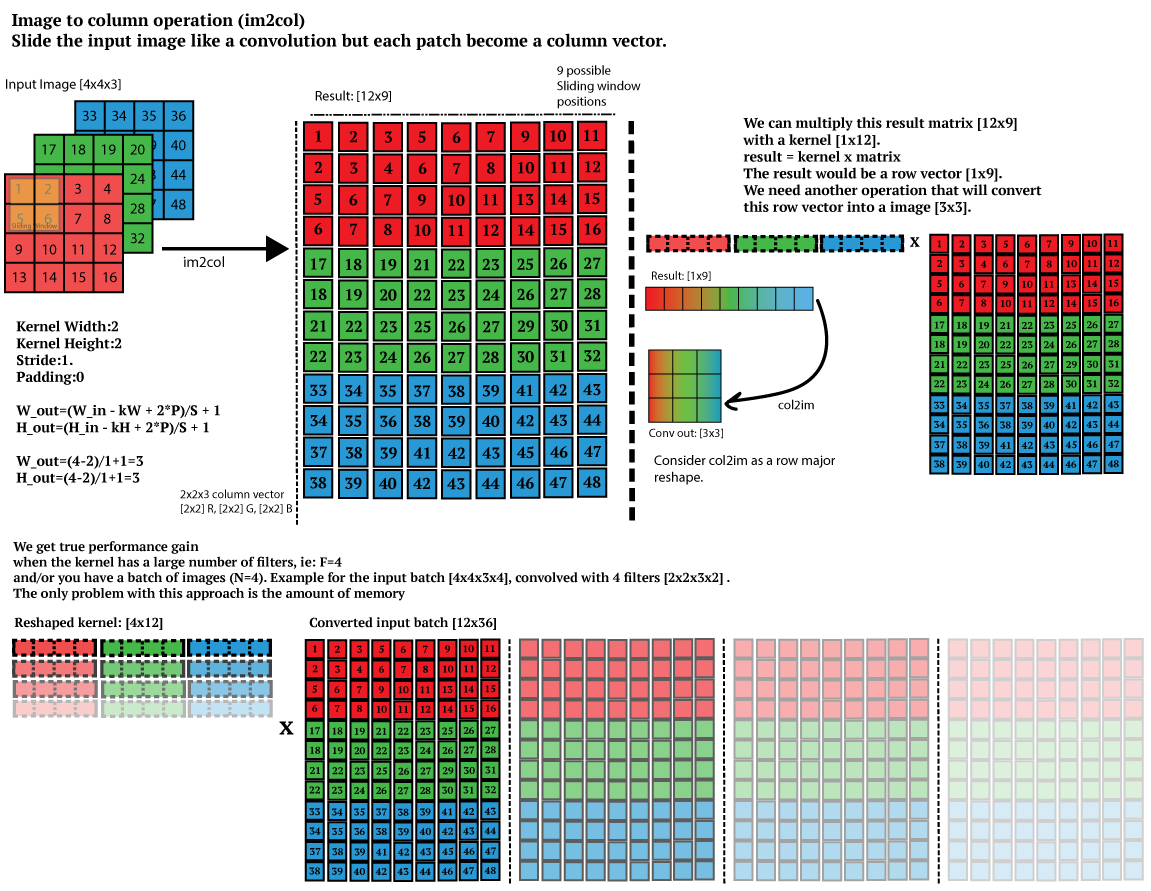
\includegraphics[width=0.85\textwidth]{im2col.png}
\caption{\textsf{im2col} algorithm scheme using a $2\times2$ filter on a image with 3 channels.
At the end of the \textsf{im2col} algorithm the \textsf{GEMM} is performed between weights and input image.
}
\label{fig:im2col}
\end{figure}
\end{center}

Taking into account what we have learned from the DNN models, we can re-formulate our problem using an efficient manipulation of the involved matrices to optimize the \textsf{GEMM} algorithm.
A direct convolution on an image of size ($W\times H\times C$), using a kernel mask of dimensions ($k \times k$), requires $O(WHCk^2)$ operations and thus several matrix products.
We can re-arrange the involved data to optimize this computation and evaluate a single matrix product: this re-arrangement is called \textsf{im2col} (or \textsf{im2row}) algorithm.
The algorithm is just a simple transformation which flats the original input into a bigger matrix, where each column carries all the elements which have to be multiplied for the filter mask into a single step\footnote{
  We work under the assumption that the weights matrix is already a flatten array and thus each row of the weights matrix represents the full mask.
}.
In this way we can immediately apply our \textsf{GEMM} algorithm on the full image.
In Fig.~\ref{fig:im2col} the main scheme of this algorithm is reported.
This algorithm optimizes the computational efficiency of the \textsf{GEMM} product but we have to store a lot of memory for the input re-organization in payback.

Using the mathematical theory behind the problem a third idea can arise using the well known Convolution Theorem: the Fourier transformation of our functions (that in this case are given by the input image and the weights kernel) can be reinterpreted into a simple matrix product in the frequency space.
This is certainly the most \quotes{physical} approach to solve this problem and probably the easier one since the Fourier Transformation is a well-known optimized algorithm, with several efficient implementations provided in literature.
One of the most efficient one is provided by the \textsf{FFTW} (\emph{Fast Fourier Transform in the West}) library~\cite{FFTW05}: \textsf{FFTW3} is an open source \textsf{Ansi-C} subroutine library for computing the Discrete Fourier Transform (DFT) in multiple dimensions, without constraints in input sizes or data types.
The library is not only computationally accurate, but it also provides an efficient parallel version for multi-threading applications.

A further implementation kind is given by linear algebra considerations (very closed to numerical considerations) and it is called \textsf{Coppersmith-Winograd algorithm}.
This algorithm was designed to optimize the matrix product and, in particular, to reduce the computational cost of its operations.
Suppose we have an input image given by just 4 elements and a filter mask with size equal to 3:

\begin{equation}
\mbox{img} = \left[\begin{array}{cccc} d0 & d1 & d2 & d3 \end{array}\right] \quad\quad \mbox{weights} = \left[\begin{array}{ccc} g0 & g1 & g2 \end{array}\right]
\end{equation}
\\
we can now use the \textsf{im2col} algorithm previously described and reshape our input image and weights into

\begin{equation}
\mbox{img} = \left[
\begin{array}{ccc}
d0 & d1 & d2 \\
d1 & d2 & d3
\end{array}
\right],
\quad\quad
\mbox{weights} = \left[
\begin{array}{c}
g0 \\
g1 \\
g2
\end{array}
\right]
\end{equation}
\\
given this data, we can simply compute the output as the matrix product of this two matrices.
The Winograd algorithm rewrites this computation as follow:

\begin{equation}
\mbox{output} = \left[
\begin{array}{ccc}
d0 & d1 & d2 \\
d1 & d2 & d3
\end{array}
\right]
\left[
\begin{array}{c}
g0 \\
g1 \\
g2
\end{array}
\right] = \left[
\begin{array}{c}
m1 + m2 + m3 \\
m2 - m3 - m4
\end{array}
\right]
\end{equation}
\\
where

\begin{equation}
\begin{aligned}
m1 = (d0 - d2)g0\quad\quad m2 = (d1 + d2)\frac{g0 + g1 + g2}{2}
\\
m4 = (d1 - d3)g2\quad\quad m3 = (d2 - d1)\frac{g0 - g1 + g2}{2}
\end{aligned}
\end{equation}
\\
where we can easily notice that the two fractions in $m2$ and $m3$ involve only weight quantities and thus they could be computed only one time for each filter (at each step).
Moreover, we have to manage $4$ \textsf{ADD} and $4$ \textsf{MUL} operations to calculate the $m_i$ quantities and $4$ other ADD to compute the result.
In doing normal matrix products we have to do $6$ \textsf{MUL} operations instead of $4$: the reduction of computational expensive \textsf{MUL} operations by a factor $1.5$x is very significant\footnote{
  A multiplication takes $7$ clock-cycles in a normal CPU while an add takes only $3$ clock-cycles.
}.
In this simple example we use a so-called $F(4, 3)$, i.e image of size $4$ and kernel of size $3$ which gives us $2$ convolutions.
More general formulations are $F(m\times m, r \times r)$ and if we use an image of size $4\times4$ and a kernel of size $3\times3$ we can compare the $16$ \textsf{MUL}s of the \textsf{Winograd} algorithm against the $36$ \textsf{MUL}s which are required by the normal matrix product ($2.25$x).
The \textsf{Winograd} efficiency has been widely proved for CNNs, especially when the kernel size is small.
In our \textsf{Byron} library we provide its implementation for kernel sizes equal to $3$, since the numerical generalization is not straightforward\footnote{
  We would also highlight that this formulation is valid only if we consider unitary strides.
}.

We tested the computational-time of each algorithm on different random images.
The tests were performed on a classical bioinformatics server (128~GB RAM memory and 2 CPU E5-2620, with 8 cores each) and we considered only kernel sizes equal to $3$ (\textsf{Winograd} constrain) varying input dimensions and number of filters.
In Fig.~\ref{fig:winograd_timing} we show the results of our simulations using the \textsf{im2col} values as reference\footnote{
  The \textsf{im2col} algorithm can be found in the major part of Neural Network library and it is also the only convolution function implemented in the \textsf{darknet} library, which is a reference for our work.
}.

\begin{figure}[htbp]
\centering
\def\svgwidth{0.8\textwidth}
\input{./img/winograd_timing.pdf_tex}
\caption{Time performances of different convolution algorithms: \textsf{im2col} (orange, reference), \textsf{FFTW3} (green, fast Fourier transformation using the \textsf{FFTW3} library) and \textsf{Winograd} (blue).
The values are normalized according to the \textsf{im2col} results since it is the most common convolution algorithm.
The tests were performed on different input sizes (width/height), keeping fixed the number of channels and the number of filters.
The tests were performed using a \textsf{C++} implementation of the three methods.
}
\label{fig:winograd_timing}
\end{figure}

In all our simulations we found a visible speedup using the \textsf{Winograd} algorithm against the other two algorithms: for small dimensions we obtained more than $5$x against the \textsf{im2col} and $25$x against the \textsf{fftw} implementation.
The worst algorithm is certainly the \textsf{fftw} one which, despite the efficient \textsf{FFTW3} parallel-library, is always more than $5$ times slower than the reference.
However, it is interesting notice how the \textsf{fftw} implementation is able to reach the best performances when the dimensions are proportional to powers of $2$, as expected from the mathematical theory behind the Discrete Fourier Transformation.

We can conclude that the \textsf{Winograd} algorithm is certainly the best choice when we have to perform a 2D convolution.
The payback of this method is given by the rigid constraints related to the mask sizes and strides: when it is possible it remains the best solution, but in all the other cases the \textsf{im2col} implementation is a relatively good alternative.
The efficiency of \textsf{Byron} library follows the efficiency of the \textsf{Winograd} algorithm, since the major part of layers in modern deep learning Neural Network models are Convolutional layers with sizes equal to $3$ and unitary strides.

%https://victorzhou.com/blog/intro-to-cnns-part-1/


\end{document}

\documentclass{standalone}

\begin{document}

\subsection[Pooling function]{Pooling function}\label{NN:pooling}

Output Neural Network feature maps often suffer of sensitivity on feature location in the input.
One possible approach to overcome this problem is to down sample the feature maps making the resulting feature map more robust to changes in the position.
Pooling functions perform this kind of down sample and they reduce the spatial dimension (but not depth) of the input.
Their use represents an important computational performance improver tool (less feature, less operations) and a useful dimensionality reduction method.
The reduction of feature quantity can also prevent over-fitting problems and it improves the classification performances.

Pooling layers are intrinsically related to Convolutional layers.
The analogy lives in the filter mapping procedure which produces the output in both methods.
While in the Convolutional layer we map a filter over the input signal and we apply a multiplication of the layer weights and the signal values, in the pooling layer we simply change the filter function keeping the same filter mapping procedure (see section~\ref{NN:convolutional} for more informations).
The input parameters of the method are the same of the Convolutional one: the input dimensions, the kernel size and (optional) the stride value.

The most common pooling layers are the Average Pool and the Maximum Pool.
The Average Pool layer performs a down sampling on the batch of images.
It slides a 2D kernel of arbitrary size over the image and the output is the mean value of the pixels inside the kernel.
In Fig.~\ref{fig:avgpool} are shown some results obtained by performing an average pool with different kernel sizes.
Also in this case this test was obtained using our NumPyNet library.

\begin{center}
\begin{figure}[htbp]
\centering
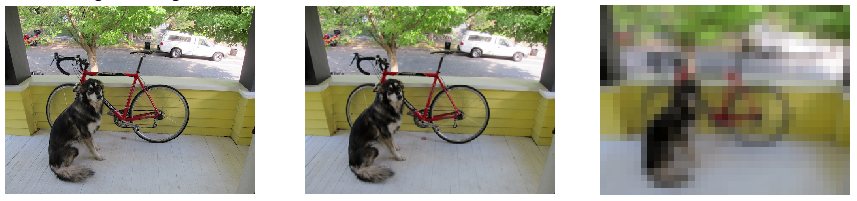
\includegraphics[width=0.85\textwidth]{avgpool_layer.png}
\caption{Average Pool functions applied on a testing image.
\textbf{(left)} The original image.
\textbf{(center)} Average Pool output obtained with a kernel mask $(3\times 3)$.
\textbf{(right)} Average Pool output obtained with a kernel mask $(30\times 30)$.
}
\label{fig:avgpool}
\end{figure}
\end{center}

If in the Convolutional layers a key role was played by the matrix product, in the Pooling layers we have to carefully manage the mapping operations to obtain optimal results.
In particular we would to show the efficient implementation provided into NumPyNet.

In the previous sections we introduced the \textsf{im2col} algorithm which is an efficient method to re-organize the input data.
The same algorithm can also be applied for Pooling layers and thus evaluate the Pooling function (avg, max, etc.) on each row of the re-arranged matrix.
The implementation of the \textsf{im2col} algorithm in Python requires the evaluation of multiple indexes using complex formulas.
Since the NumPyNet library was founded on the Numpy package we can provide an alternative implementation using the \textsf{view} functionality of the library.
A \textsf{view} of a given array is simply another way of viewing its data: technically that means that the data of both objects is shared and thus no copies are created.
In particular we can use the deeper functions of the Numpy package to create a re-organization of our data according to the desired output\footnote{
  The same technique was also used for the implementation of the Convolutional layer in the NumPyNet library.
}.
In the following code we show our implementation of the Average Pooling layer:

\lstset{style=snippet}
\begin{lstlisting}[language=Python, caption=NumPyNet version of AvgPool function, label=code:py_avgpool]
import numpy as np

class Avgpool_layer(object):

  def __init__(self, size=(3, 3), stride=(2, 2)):

    self.size = size
    self.stride = stride
    self.batch, self.w, self.h, self.c = (0, 0, 0, 0)
    self.output, self.delta = (None, None)

  def _asStride(self, input, size, stride):

    batch_stride, s0, s1 = input.strides[:3]
    batch,        w,  h  = input.shape[:3]
    kx, ky     = size
    st1, st2   = stride

    # Shape of the final view
    view_shape = (batch, 1 + (w - kx)//st1, 1 + (h - ky)//st2) + input.shape[3:] + (kx, ky)

    # strides of the final view
    strides = (batch_stride, st1 * s0, st2 * s1) + input.strides[3:] + (s0, s1)

    subs = np.lib.stride_tricks.as_strided(input, view_shape, strides=strides)
    # returns a view with shape = (batch, out_w, out_h, out_c, kx, ky)
    return subs

  def forward(self, input):

    self.batch, self.w, self.h, self.c = input.shape
    kx, ky = self.size
    sx, sy = self.stride

    input = input[:, : (self.w - kx) // sx*sx + kx, : (self.h - ky) // sy*sy + ky, ...]
    # 'view' is the strided input image, shape = (batch, out_w, out_h, out_c, kx, ky)
    view = self._asStride(input, self.size, self.stride)

    # Mean of every sub matrix, computed without considering the pad(np.nan)
    self.output = np.nanmean(view, axis=(4, 5))

\end{lstlisting}

A key role in this implementation is played by the \textsf{\_asStride} function: it returns a view of the original array in which all the masks are organized into a single list.
Using this data re-arrangement we can easily compute the desired pooling function (average in this example) according to the appropriated axes.
We would stress that no copies are produced during this computation and thus we can obtain a faster execution than other possible implementations (e.g \textsf{im2col}).

\end{document}

\documentclass{standalone}

\begin{document}


\section[BatchNorm function]{BatchNorm function}\label{batchnorm}

A common practice before the training of a Neural Network model is to apply some preprocessing to the input patterns.
A classical example is the normalization of training set, i.e it resembles a normal distribution with zero mean and unitary variance.
The initial preprocessing is useful to prevent the early saturation of non-linear activation functions (see section~\ref{activation}).
Moreover in this case we can ensure that all inputs are in the same range of values.

In a deep neural network architecture we can find the same problem also into the intermediate layers because the distribution of the activations is constantly changing during training.
This behavior produces a slowdown in the training convergence because each layer have to adapt itself to a new distribution of data in every training step (or \emph{epoch}).
This problem is also called \emph{internal covariate shift}.

A second problem arises from the heterogeneity of available input data.
If we tune the model parameters according to a given set of data which inevitably be limited we can meet problems during the generalization, i.e the validation of our model using new data, to new samples if they belongs to an equivalent but deformed distribution.
A classical example is given by the image detection: if we train a Neural Network model using gray-scale images we can find generalization problem using colored images.

BatchNorm function (Batch Normalization) allows to overcome these problems with a continuous rescaling of the Neural Network intermediate values during the training\footnote{
  The input data to feed the Neural Network model are commonly packed into a series of \emph{batches}, i.e small subsets of data.
  The BatchNorm function takes its name from this nomenclature and it processes each batch independently.
}~\cite{Sergey2015BatchNorm}.
In particular, the method processes the input of a given layer in order to fight the internal covariate shift problem removing the batch mean and normalizing by the batch variance:

$$
\mu_B = \frac{1}{m}\sum_{i=1}^{m}x_i \quad\quad {\sigma_B}^2 = \frac{1}{m-1}\sum_{i=1}^{m}(x_i - \mu_B)^2
$$
\\
and so the input data becomes:

$$
\hat{x_i} = \frac{x_i - \mu_B}{\sqrt{{\sigma_B}^2 + \epsilon}}
$$
\\
where we add an extra $\epsilon$ in the denominator for numerical stability\footnote{
  The floating point numbers into a computer have finite precision and the variance can underflow bringing to infinite values in the BatchNorm equation.
}.
After this common rescaling we also a apply a scaling-shift to previous results:

$$
y_i = \gamma\hat{x_i} + \beta
$$
\\
where the $\gamma$ and $\beta$ coefficients are left as variables to be tuned during the training (they are learned during training).
The updating rule of the function parameters ($\gamma$ and $\beta$) is given by the simple derivative of the previous function. % maybe insert backprop formulas
In this way we can ensure more stability of the extracted features~\cite{Lecun2000EffBackProp} during the training a faster convergence.

Since the BatchNorm function is became a sort of standard into a deep learning models an efficient implementation of this algorithm is essential to achieve the best computational performances.
We have also to take in count that the batch-normalization procedure is commonly performed after a fully-connected layer or a convolutional one.
Thus the best performances could be obtained merging the two functionality as much as possible as suggested in~\cite{AlexeyAB}.
In the next sections we will show our implementation of the algorithm and we discuss about the code optimization performed\footnote{
  The Byron library was inspired by the \emph{darknet} library provided by Redmon J. et al. and by its many branches.
  Despite in each implementation we can find the BatchNorm function, aware of the author, in any version we can find a right implementation of this function as standalone method.
  We have already highlighted that this normalization function can be efficiently joined to other function to increase the computational performances but in these case we have to different manage the dimensions of the involved arrays.
  A standalone implementation of the BatchNorm function required a rearrangement of its functions and it was provided into the Byron library.
  This was one of the various improvements provided by Byron against the other \emph{darknet}-like libraries.
}.

\end{document}

\documentclass{standalone}

\begin{document}


\section[Shortcut]{Shortcut function}\label{shortcut}


\end{document}

\documentclass{standalone}

\begin{document}


\section[Route]{Route function}\label{route}

\end{document}



\documentclass{standalone}

\begin{document}

\section[NumPyNet]{Neural Network laboratory - NumPyNet}\label{numpynet}

%Description of the Neural Network laboratory developed in pure numpy.
%Study of the neural network functionality.
%Testing of the code against tensorflow.



\end{document}
 % Introduction to NumPyNet

\documentclass{standalone}

\begin{document}

\section[rFBP]{Replicated Focusing Belief Propagation}\label{rfbp:rfbp}

Up now we have implicitly talked about Neural Network models based on the standard updating rule of back-propagation.
Other learning rule for weight updates were proposed and the choice of the best one it is still an open-problem.
The final purpose is to obtain a feasible learning rule ables to model the biological learning of the human brain.

The learning problem could be faced through statistical mechanic models joined with the so-called Large Deviation Theory.
In general, the learning problem can be split in two sub-parts: the classification problem and the generalization one.
The first aims to completely store a pattern sample, i.e a prior known ensemble of input-output associations (\emph{perfect learning}).
The second one corresponds to compute a discriminant function based on a set of features of the input which guarantees a unique association of a pattern.

From a statistical point-of-view many Neural Network models have been proposed and the most promising seems to be spin-glass models based.
Starting from a balanced distribution of the system, generally based on Boltzmann distribution, and under proper conditions, we can prove that the classification problem becomes a NP-complete computational problem.
A wide range of heuristic solutions to that type of problems were proposed.

In this section we show one of these algorithms developed by Zecchina et al.~\cite{BaldassiE7655} and called \emph{Replicated Focusing Belief Propagation} (rFBP).
The theoretical background of the algorithm is beyond the scope of this thesis so we focus on its numerical implementation and optimization.

Moreover, despite their proved theoretical efficiency, the applications on real data are still few.
Thus, we show the application of the optimized version of the rFBP algorithm on a Genome Wide Association (GWA) dataset provided by the European \href{https://www.compare-europe.eu/}{COMPARE project}.
This work was also presented on the 2019 CCS-Italy (Conference of Complex System)~\cite{DallOlioCCS19}.

\end{document}

\documentclass{standalone}

\begin{document}


\subsection[Algorithm Optimization]{Algorithm Optimization}\label{rfbp:rFBP}

The rFBP algorithm is a learning algorithm developed to justify the learning process of a binary neural network framework.
The model is based on a spin-glass distribution of neurons put on a fully connected neural network architecture.
In this way each neuron is identified by a spin and so only binary weights (-1 and 1) can be assumed by each entry.
The learning rule which controls the weight updates is given by the Belief Propagation method.

A first implementation of the algorithm was proposed in the original paper~\cite{BaldassiE7655} jointly with an open-source Github repository.
The original version of the code was written in Julia language and despite it is a quite efficient implementation the Julia programming language stays on difficult and far from many users.
To broaden the scope and use of the method, a C++ implementation was developed with a joint \emph{Cython} wrap for Python users.
The C++ language guarantees better computational performances against the Julia implementation and the Python version enlarge its usability.
This implementation is optimized for parallel computing and is endowed with a custom C++ library called \emph{Scorer} (see Appendix D for further details), which is able to compute a large number of statistical measurements based on a hierarchical graph scheme.
With this optimized implementation we try to encourage researchers to approach these alternative algorithms and to use them more frequently on real context.

As the Julia implementation also the C++ one provides the entire rFBP framework in a single library callable via a command line interface.
The library widely uses template syntaxes to perform dynamic specialization of the methods between two magnetization versions of the algorithm.
The main object categories needed by the algorithm are wrapped in handy C++ objects easy to use also from the Python interface.
A further optimization is given by the reduction of the number of available functions: in the original implementation a large amount of small functions are used to perform a single complex computation step, enlarging the amount of call stack; in the C++ implementation the main functions are re-written with the minimizing the call stack to ease the vectorization of the code.

The full rFBP library is released under MIT license and it is open-source on Github~\cite{ReplicatedFocusingBeliefPropagation}.
The on-line repository provides also a full list of installation instructions which could be performed via \emph{CMake} or \emph{Makefile}.
The continuous integration of the project is guaranteed in every operative system using \emph{Travis CI} and \emph{Appveyor CI} which test more than 15 different C++ compilers and environments.

The Python wrap guarantees also a good integration with the other common Machine Learning tools provided by \emph{scikit-learn} Python package; in this way we can use the rFBP algorithm as equivalent alternative also in other pipelines.
Like other Machine Learning algorithm also the rFBP one depends on many parameters, i.e its hyper-parameters, which has to be tuned according to the given problem.
The Python wrap of the library was written according to \emph{scikit-optimize} Python package to allow an easy hyper-parameters optimization using the already implemented classical methods.


\begin{figure}[htbp]
\centering
\def\svgwidth{0.85\textwidth}
\input{./img/rfbp_magp_timing.pdf_tex}
\caption{Comparison of time performances between the original Julia implementation and our Cython one of the rFBP algorithm varying the input dimension sizes (number of samples, $M$, and number of variables, $N$).
For each input configuration 100 runs of both algorithm were performed and the results were normalized by the Julia implementation.
In these cases we fixed the magnetization to \textbf{MagP64}.
}
\label{fig:rfbp_magp}
\end{figure}

\begin{figure}[htbp]
\centering
\def\svgwidth{0.85\textwidth}
\input{./img/rfbp_magt_timing.pdf_tex}
\caption{Comparison of time performances between the original Julia implementation and our Cython one of the rFBP algorithm varying the input dimension sizes (number of samples, $M$, and number of variables, $N$).
For each input configuration 100 runs of both algorithm were performed and the results were normalized by the Julia implementation.
In these cases we fixed the magnetization to \textbf{MagT64}.
}
\label{fig:rfbp_magt}
\end{figure}
%30 (N,M) con N in 1001-5001 con 1000, M=101-351 con 50 ognuna 100 magT

We firstly test the computational efficiency of our implementation against the original Julia one.
The tests were performed comparing our \emph{Cython} version of the code (and thus with a slight overhead given by the Python interpreter) and the Julia implementation as reference.
Varying the dimension sizes (number of samples, $M$, and number of variables, $N$) we tested the time efficiency over 100 runs of both the algorithms.
We divided our simulation according to the two possible type of magnetizations (MagP64 and MagT64 as described by the original implementation available \href{https://github.com/carlobaldassi/BinaryCommitteeMachineFBP.jl}{here}) and the obtained results are shown in Fig.~\ref{fig:rfbp_magp}~\ref{fig:rfbp_magt}, respectively.

As can be seen by the two simulations our implementation always overcome the time performances of the original one, taken as reference in the plot.
However, we can not guarantee a perfect parallel execution of our version: also with multi-threading support the scalability of our implementation does not follow a linear trend with the number of available cores.
In our simulation, in fact, we used 32 cores against the single thread execution of the Julia implementation but we gained only a 4x and 2x of speedup for MagT64 and MagP64, respectively.
The network training is a sequential process by definition and thus it is hard to obtain a relevant speedup using a parallel implementation.
In this case it is probably jointed to a not perfect parallelization strategy chosen which bring to a not efficient scalability of our algorithm version.
However, the many improvements performed to the code allow us to use this algorithm with bigger dataset sizes.

\end{document}

\documentclass{standalone}

\begin{document}


\subsection[Compare dataset]{SNP classification}\label{rfbp:snp}

The few available applications of the rFBP algorithm to real data are amenable to two aspects: I) learning technique; II) algorithm implementation.
The first one is related to the intrinsic definition of the algorithm which is designed to reach a complete memorization of the training dataset; in the other Machine Learning processes we normally want to avoid this kind of results since it could bring to \emph{over-fitting} problems.
The second one is given by the binary values involved in each step of the algorithm which intrinsically limit the possible applications\footnote{
  The Neural Network weights can assume only binary values since they model up/down spins.
  Moreover also the input is required to be a spin configuration and thus binary.
  The common Machine Learning problems involve floating-point values as input pattern.
}.


Classification problems which involved only binary quantities are quite small but the GWA is one of them.
In the GWA we have a series of genome data belonging to different classes as input.
A genome is the ensemble of genes of an organism and each gene is identified by a series of nucleotides with 4 possible values (G, guanine; C, cytosine; A, adenine; T, thymine).
The comparison between a reference (healthy) genome and an infected one highlights the biological mutation related to the understudy disease.
This mutation are the so-called SNPs (Single Nucleotide Polymorphisms).
So we can identify a genome as a sequence of its mutation in relation to a reference genome, i.e a sequence of two possible values given by the on/off of the mutation in each nucleotide.

The COMPARE project aims to develop new methods to avoid the genetic disease transmission.
In this project plays a crucial role the \emph{Source Attribution}, i.e the classification of a given disease based on the list of its mutation.

We tested the rfBP on $210$ Salmonella enterica genome sequences, $4857450\,bp$ (base pairs) long, living inside animals.
Our early goal was to discriminate those bacteria living in pigs (159 samples) with respect to all the others animals (51 samples).

First of all we filter our data removing from each genome a base if it is not mutated in each sample.
In this way we reduce the number of bases to $8189\,bp$.
A graphical representation of these samples is given in Fig.~\ref{fig:SNPsAle}.
The dataset was divided in training and test sets using a stratified cross-validation procedure to guarantee a proportional subdivision of the samples into the two classes.
The algorithm hyper-parameters was tuned on the training set based on the performances obtained using a internal stratified 10-fold cross-validation: in each fold the training was performed by a given sequence of hyper-parameters and the performances evaluated on the corresponding test set; the hyper-parameters configuration which obtains the best performances on the full training set was chosen as best configuration.
The performances evaluation was performed using the custom \emph{Scorer} library.
Considering the unbalanced sample quantities the Matthews Correlation Coefficient (MCC) is chosen as good scorer indicator for the evaluation.

With the tuned hyper-parameters we performed the training of rFBP algorithm on different percentage of the training set: $25\%$, $45\%$, $65\%$ and $85\%$.
In the same way we train also a list of the most common Machine Learning classifiers: single perceptron with floating-point weights (Perc); standard Neural Network with gradient descent as updating rule (MLP); support vector machine with linear kernel (lSVM); support vector machine with radial kernel (rSVM); linear discriminant analysis (LDA); decision tree (DT); random forest (RF); k-nearest neighbors with 2-clusters (kNN); Guassian process (GP); diag-quadratic discriminant analysis (GNB); Bernoulli naive bayes (BNB); AdaBoost (AdaB).
For each training percentage we perform the optimization of the hyper-parameters of each classifier with the same number of optimization steps.
In Fig.~\ref{fig:confronto_bestclassificatoriACC, fig:confronto_best_classificatoriMCC} the accuracies and MCC results are shown, respectively.

From this analysis we can conclude that the rFBP algorithm shows comparable performances with the other classifiers.
These performances globally grow with the training set size but only the rFBP is able to reach a \quotes{perfect learning} configuration, i.e accuracy of 100\% and MCC=1.
We have also noticed that the rFBP classifier and the GNB are the only two algorithms which qualitatively does not show performances saturation on their training.

A second analysis was performed on the data distribution using a multiple $\chi^2$-test.
Starting from the whole set of genomes we can compute the contingency-matrix of the two classes\footnote{
  The contingency-matrix displays the (multivariate) frequency distribution of the variables.
  Each row will count the number of hosts with/without the SNPs.
  Each column will identify a class.
}.
The $\chi^2$-test was performed on the full set of $8189\,bp$ and so the extracted \emph{p-values} were corrected according multiple-tests.
Using the \v{S}id\'ak~\cite{Sidak1967} correction method and by the definition of significant threshold of $0.05$ we found $1103$ significant bases.
An analogous $\chi^2$-test was performed on the rFBP weights to identify a putative

% MISS

\end{document}

\documentclass{standalone}

\begin{document}


\section[Conclusion]{Conclusion}\label{snp_conclusion}



\end{document}


\documentclass{standalone}

\begin{document}

\section[Byron]{Build YouR Own Neural network - Byron library}\label{byron}

Limits of the most common neural network frameworks.
Neural Network library for parallel computing developed in C++.
Pyron as python wrap of the library.
Description of the algorithms used to optimize the computation (ex. im2col vs winograd).


\end{document}


\documentclass{standalone}

\begin{document}

\section[Object Detection]{Object Detection}\label{obj_detection:obj}

Object detection is one of the larger deep learning sub-discipline, especially when we talk about Neural Network models.
This kind of problems aim to identify single or multiple objects into a picture or video stream.
The possible applications of these tools are everywhere these days and they involve object tracking, video surveillance, pedestrian detection, anomaly detection, people counting, self-driving cars or face detection and the list goes on.

There are many machine learning and deep learning techniques proposed during the years about this topic and each one has its own pros and cons.
The most prominent and moder techniques involve the use of very deep Neural Network models, with a huge amount of parameters to tune.
The most famous ones are probably the Faster R-CNN (\emph{Faster Region Convolutional Neural Network})~\cite{ren2015faster} and its \quotes{evolution} into the YOLO (\emph{You Only Look Once}) model~\cite{redmon2015look, redmon2016yolo9000, redmon2018yolov3}.

The R-CNN models are one of the state-of-art CNN-based deep learning object detection model and their evolution into Fast R-CNN tries to improve their speed.
The standard approach for object detection is based on moving a \emph{sliding window} to search in every position of the image the objects.
However, the intrinsic problems of these kinds of methods are the window dimensions and the large computation required to map with multiple window sizes the full image.
Different objects, or even the same kind of objects, could have different aspect ratios and sizes in relation to the position of the camera which captured the image or to their distances.
R-CNN models try to overcome these problems generating about \numprint{2000} region proposals, i.e bounding boxes, and applying to each one a image classification procedure, using a standard CNN.
Finally, each detected region can be refined using a regression approach.

A Faster R-CNN model is based on the same idea but, instead of feeding the bounding boxes to the CNN, it feeds the input image to the CNN to generate a convolutional feature map.
Starting from this feature map we can easier identify the region of proposals (Region Proposal Network) and warp them into squares.
The list of these regions are then reshaped using a Polling layer and processed by a fully connected layer.
The advantages of Faster R-CNN are thus visible: we do not need to feed \numprint{2000} region proposals to the CNN every time, but the feature map is generate once per image using the convolution operation.
In this way we can also separate the feature map creation to the selective search algorithm.

A key role on these models is given by the \emph{anchor} concept: an \emph{anchor} is essentially a box and it identifies the shape of a portion of the input image at different scale levels.
The CNN feature map feeds the Region Proposals Network which uses a sliding window over it, generating $k$ anchor boxes.
These boxes are certainly fewer than the previous cited \numprint{2000} windows.

A breakthrough idea on the real-time object detection was the introduction of the YOLO model.
The model was developed by Redmon et al. at Washington University and it is probably the state-of-art on object detection, especially for its very incredible speed (it can reach 45 FPS on modern GPUs!).
Certainly it is the faster method publicly available, but its popularity is also due to its innovative strategy in object detection.
Despite all the other algorithms use regions to localize the object into the image, the YOLO network does not look at the complete image but only on a parts of it, which has the higher probability to contain an object.
In YOLO a single CNN predicts the bounding boxes and the class probabilities of them.
YOLO slits a single image into a $S\times S$ grid and on each grid $m$ bounding boxes are taken.
For each of them, the CNN outputs a class probability and offset values.
Finally, these bounding boxes are filtered according to their probability and a chosen threshold.

One of the most bigger limitation of this model is that it struggles with small objects.
This is due to the spatial constraints of the algorithm.
Fortunately, in the previous sections we have already discussed on how we can overcome this kind of problem using Super Resolution.
In the next section we will discuss about further characteristics of the YOLO model and about its implementation into the \textsf{Byron} library, considering its efficiency against the original implementation.
Finally, we will join the efficiency of the previous Super Resolution models to the performances of our optimized implementation of YOLO.


%Introduction on the image classification and detection with Yolo architecture.
%Implementation in Byron with description of performances against darknet (original implementation).
%Focus on performances (time, memory, cpu).


\end{document}


\documentclass{standalone}

\begin{document}

\section[Super Resolution]{Super Resolution}\label{SR:sr}

\begin{figure}[htbp]
\def\svgwidth{0.5\textwidth}
\input{./img/sr_wow.pdf_tex}
\quad
\def\svgwidth{0.465\textwidth}
\input{./img/sr_wow2.pdf_tex}
\caption{Single Image Super Resolution.
Between the red lines the super resolved version of the original image.
}
\label{fig:sr_wow}
\end{figure}

The Super Resolution (SR) is a slight novel technique based on Neural Network models which aims to improve the spatial resolution of a given image\footnote{
  The best-known \quotes{implementation} of Super Resolution concerns the microscopy super-resolution.
  In this work we are focusing on algorithms and numerical implementations so we will talk about the numerical counterpart of this technique, totally ignoring the original \quotes{hardware} version.
}.

The first SR methods on digital images estimate the high frequency information of the images, starting from a series of low-resolution (LR) patches and their high-resolution (HR) counterparts.
These patches (ROIs of the LR image commonly smaller than $50\times50$) were extracted after an edge enhancement procedure or a simple 2D Fourier transformation, which extracts the high frequency information.
Collecting these patches an \quotes{association dictionary} between LR and HR was created.
This dictionary was used to learn the correct associations between LR and HR and then applied on new images.
The images considered were of the same dimensions in these firstly applications, i.e the purpose was only to improve the spatial resolution of the image without changing the sampling step.

The idea of use neural network models and in particular convolution functions to face this problem was born in 2014 at the Engineering University of Honk Kong, due to the large popularity of these models during those years.
The increasing computational power allowed to create automatic models able to learn the LR-HR associations without any dictionary.
In this year the SRCNN model~\cite{SRCNN} arises, a three-layer neural network able to learn a large ensemble of features to reproduce the desired associations.
The first layer aimed to extract the LR patches from the input image; the second layer produces the association between the LR patches and the tuned HR ones; the last layer reorganized the HR patches ensemble produced into a single HR image, i.e the output.

From this starting implementation many improvements was performed in this research field, but the fundamental idea is not changed.
Modern models simply have a greater number of layers, due to the increasing computational power availability, and they use appropriated workaround to overcome the (large-)parameters tuning problem.

In the next sections we will show the super resolution technique step-by-step starting from the image pre-processing up to the most modern algorithmic solutions.
At the end of this chapter the \textsf{NumPyNet} and \textsf{Byron} implementations of some modern models will be presented and applied over biomedical images.

%Introduction on Super Resolution problem with focus on state-of-art neural network architecture.
%Description of the Byron implementation and application on NMR data with the most common measurements.
%Super-resolution allows better detection!


\end{document}


\documentclass{standalone}

\begin{document}

\section[Segmentation]{Image Segmentation}\label{segmentation:unet}

\begin{center}
\begin{figure}[htbp]
\centering
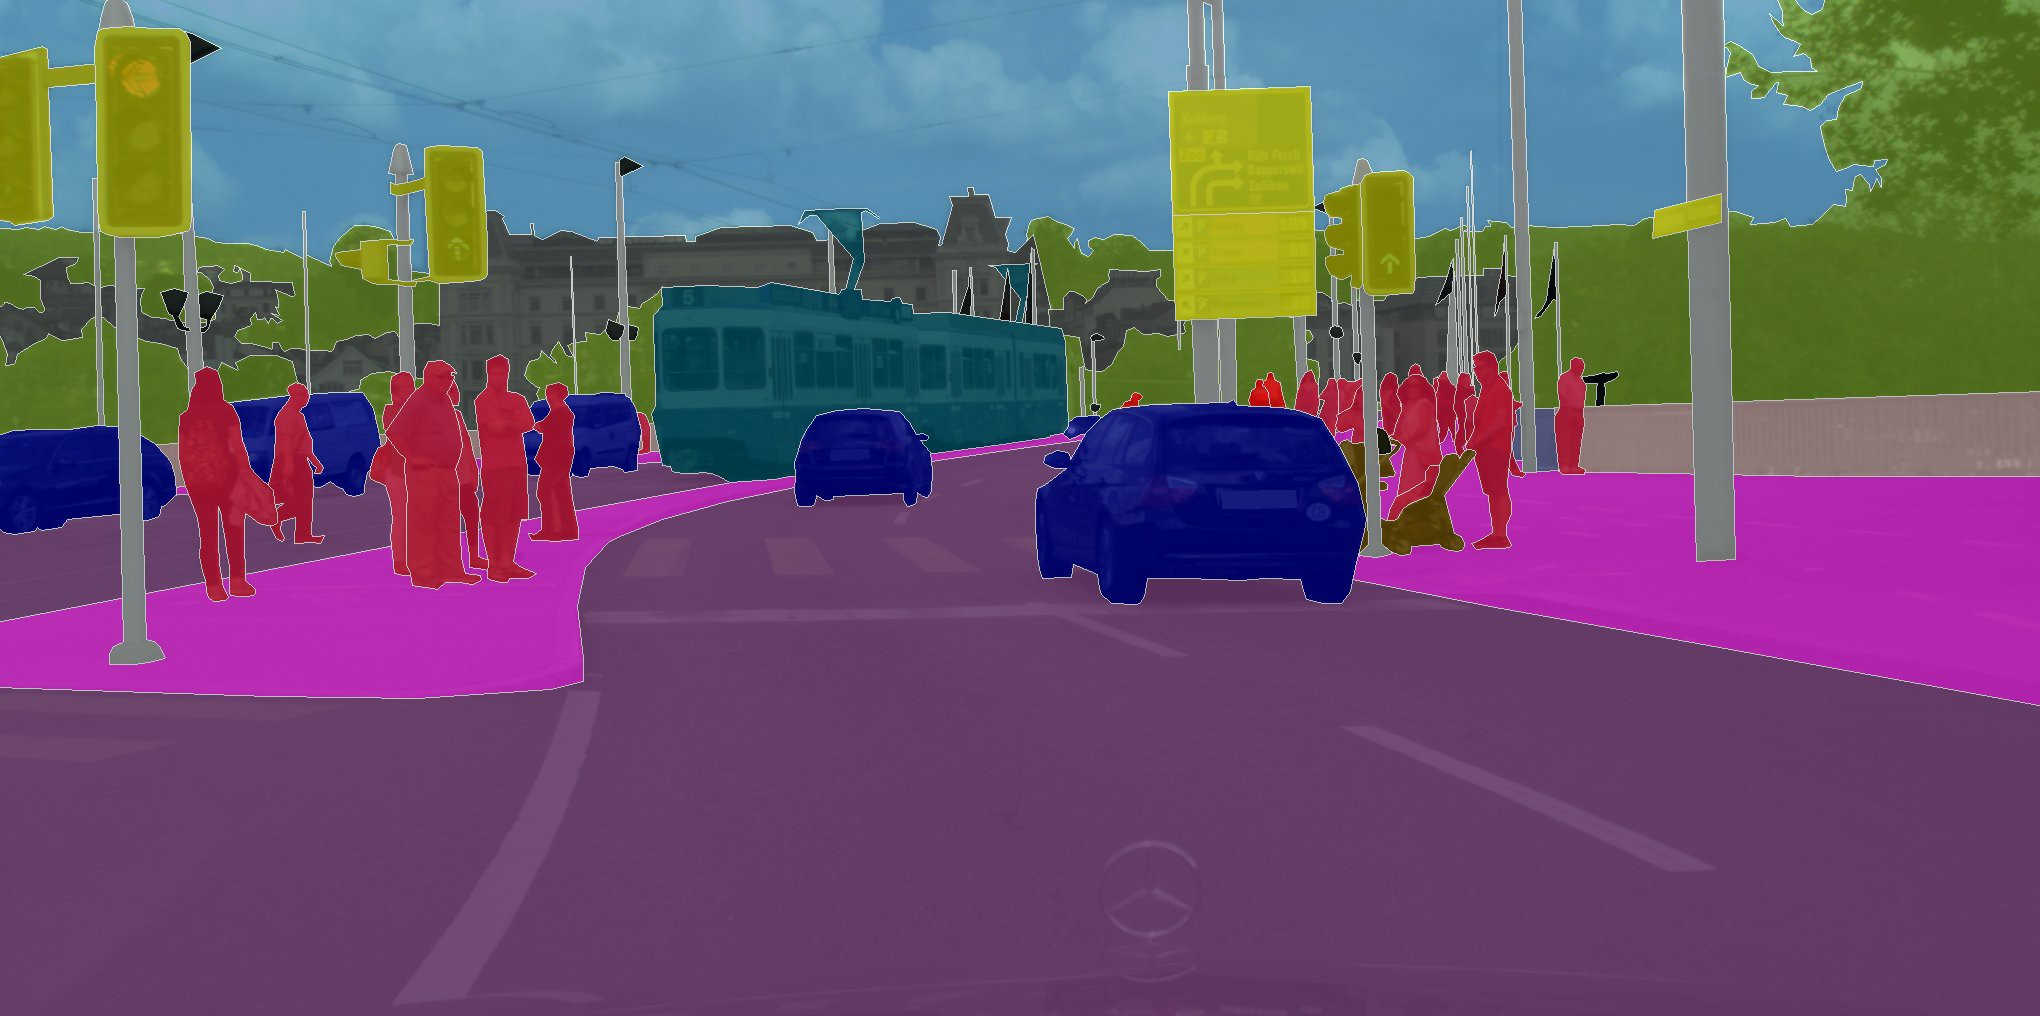
\includegraphics[width=0.85\textwidth]{segmentation.jpg}
\label{fig:segmentation}
\end{figure}
\end{center}

In the previous section we have discussed about the object classification and object detection problems (ref.~\ref{obj_detection:obj}).
Now we want to go deeper on this topic and extract the exact pixels which belong to an object into a given image.
This kind of problem is called Image Segmentation, i.e give a label to each pixel of the input image.

Image segmentation is a typical task in many research fields and could be used for different purposes.
information about pixel-wise position of objects inside an image could be used for extract object shapes from the image or to simplify and/or change the representation of an image into something more meaningful and easier to understand.
This is an hot topic especially for self-driving car applications in which we have to find the exact shapes of object to better estimate their perspective position.
Moreover, all these applications require fast algorithm as much as possible closed to real-time.

This kind of task can be performed using a pipeline of image processing functions or by training a neural network model.
In the first case we have to stack a series of function to process the input image: it has to filters and extracts the useful information about the searched object but most of all it has to be as most general as possible to face on the common heterogeneity of samples.
In the second case we leave to the neural network model parameters the searching of optimal combination of function but we have to provide a supervised input pattern, i.e a combination of input and annotated pixel-wise mask of each image.
The image annotation is one of the most hardest and boring step of image segmentation and for these reasons is very hard to find public dataset usable.

In this chapter we introduce a particular neural network model commonly used in image segmentation problems and we will describe its characteristics and performances.
We applied this model to a novel dataset of CT images.
The dataset annotation was performed by a custom semi-supervised pipeline of image processing and the neural network model was trained and tested on this dataset.
The original data are taken from \href{}{here} and the corresponding annotations are released on \href{}{here}.

\end{document}



\end{document}
